%Bemerkung: Diese Datei wird über den \input{<name>.tex} in einer anderen .tex Datei %eingebunden. Daher müsst ihr euren Kram einfach nur noch runterschreiben
%Beispielsweise: 
\section{Software - Design}
\subsection{Usecases}
The flying software is definied by 12 different usecases and three actors. \\ \\
The Controller actor represents the most complex actor system in this project. It uses the Analog Digital Converter (ADC) of the STM32F779 Controller and six external ADC to measure the temperature or the resistance of the twelve strain gauges. \\ \\ 
The usecase \textit{ADC external Request} describes the SPI communication to the six external ADCs. One ADC is used for two channels, there will be one pyhsical strain-gauge per ADC. Each strain-gauge has a $X$, $Y$ channel. The strain-gauge channels are splitted so each channel of them is connected to one channel at the ADC. Therefore each channel is sampled with  1 kSPS (Sample Per Second). \\ \\
The second ADC usecase \textit{ADC Internal Request} is for sampling the temperature from six PT-100 sensors. The sampling will be done by the internal 12 bit ADC from the STM32F779. Therefore its enugh to sample with 20 SPS. \\ \\
\textit{Telemetry} covers each communication with the REXUS Serivce Module. It includes the \textit{Error Handling} and \textit{Compression} usecase. Each time the microcontroller ($\mu C$) sends something to its ground station, this usecase is called. After each transmission, the REXUS Service Module will return the error rate. So the telemetry has to adjust thier speed to maintain a soild communication. \\ \\
The \textit{Memory Usage} usecase describes how the memory is used. It is called each time the $\mu C$ saves something to flash memory. The controller have to save each measurment result and meta information about the flight, communication quality and in-flight problems. This usecase also includes \textit{Compression}, \textit{Write To Memory}, \textit{Reset Memory} and \textit{Read From Memory}. It is extended by the \textit{USB} usecase, this is for memory usage to get all  measurement result from memory. \\ \\ 
\textit{Debug}, this usecase describes the communication from Ground Station Software to the Controller. Therefore will be an JTAG interface implemented, connected via \textit{USB}. In pre-flight it will be used to gather information about the mechanical testcases. This usecase includes \textit{USB} as a hard connection  between this two usecases. \\ \\
The \textit{DAPI} for \textit{D}ata \textit{a}nd \textit{p}rogramming  \textit{i}nterface usecase, describes the communication from ground station software to the microcontroller. It extendes the \textit{USB} usecase.\\ \\
See Figure \ref{fig:usecase} as reference. 
\pagebreak
\begin{figure}[H]
	\centering
	  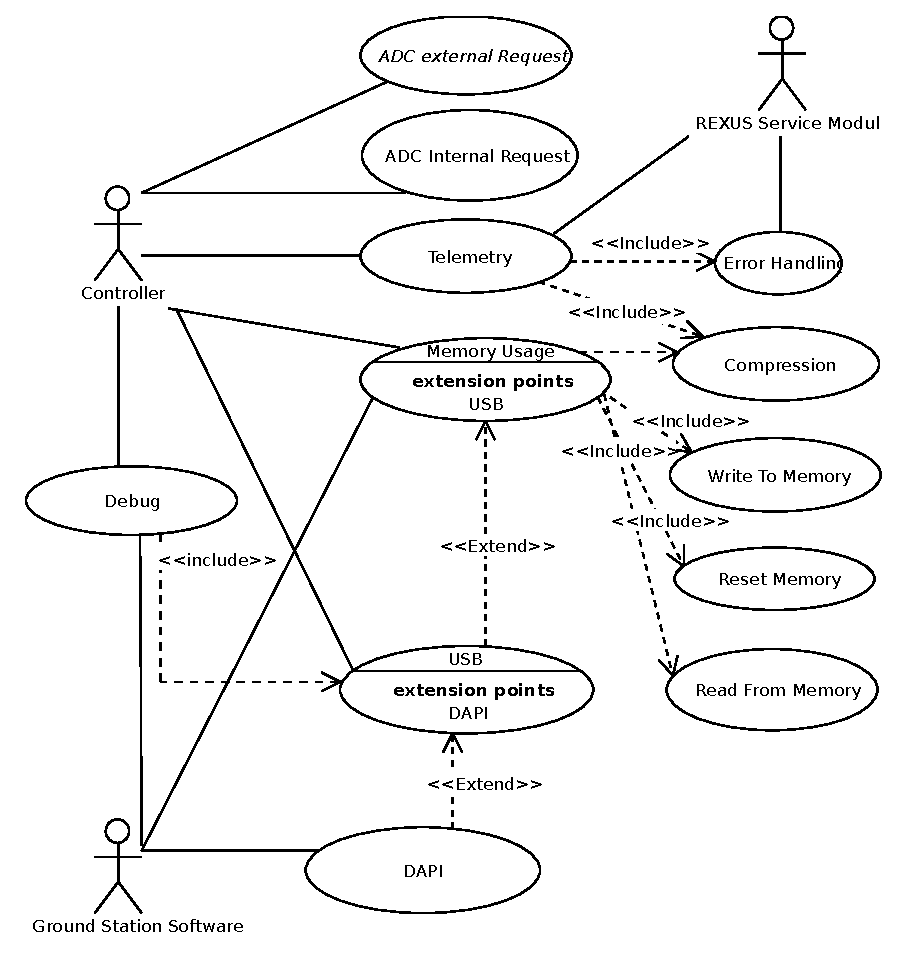
\includegraphics{HERMESS_USECASE.eps}
	\caption{Usecases}
	\label{fig:usecase}
\end{figure}
\pagebreak
\begin{figure}[H]
	\centering
	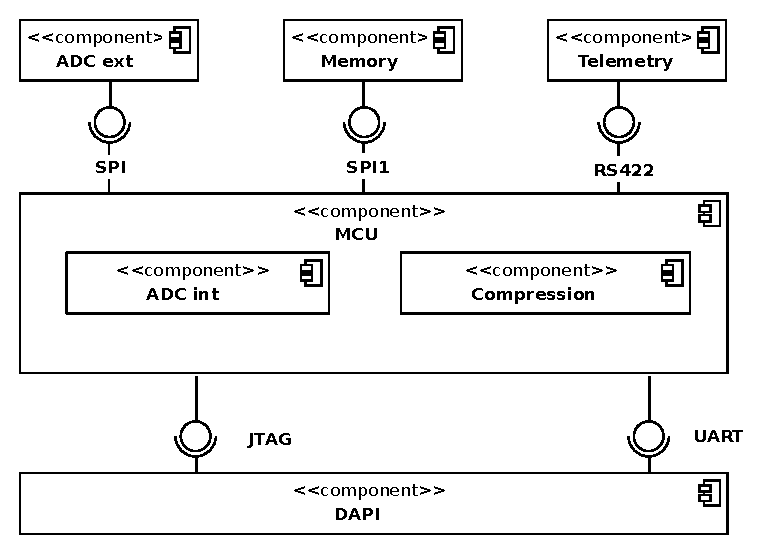
\includegraphics{Components.eps}
	\caption{Component Diagramm}
\end{figure} \noindent
The components are \textit{ADC ext}, \textit{ADC int}, \textit{Memory}, \textit{Telemetry}, \textit{MCU}, \textit{Compression} and \textit{DAPI}. There five communication interfaces two of them are \textit{SPI}, one time \textit{RS422}, \textit{JTAG} and \textit{UART}.\\ \\
The component \textit{ADC ext} describes the communication with the external ADCs. This communication is SPI bases and works via chip select. There are three diffrerent SPI each of them is communicating with two ADCs. \\ \\
The \textit{Memory} component  describes two 128 Mbyte flash memory blocks each of then  is conntect to its own SPI. There is not a memory concept yet. \\ \\
The \textit{Telemetry} component is the onboard REXUS Service Module, the communication will be maintained by a RS422 interface. \\ 
Component \textit{MCU} descibes the main controller, all components execpt the external ADC, Telementry, DAPI and Memory are not implmeneted on this MCU. The MCU provides and describes the interfaces used for communication. The internal communication with the internal ADC will be done by Direct Memory Acces (DMA). The processing of measurment result will be done by message queues. Message queues are also used to interthread communication. \\ 
The \textit{DAPI} component is conntect to the \textit{MCU} by two diffrent interfaces. At first it is used to programm the \textit{MCU} via \textit{JTAG}. Second it is communicating with the \textit{MCU} via UART at a BAUD rate about 115200, 8, n 1 for memory usage and system maintance. 